\documentclass{senior-design}

%%% Fonts %%%%%%%%%%%%%%%%%%%%%%%%%%%%%%%%%%%%%%%%%%%%%%%%%%%%%%%
\setmonofont[Scale=MatchLowercase]{Consolas}
\setsansfont{Arial}
\usepackage{newpxtext, newpxmath} % Palatino
\graphicspath{{Figures/}}
%%% Report information %%%%%%%%%%%%%%%%%%%%%%%%%%%%%%%%%%%%%%%%%%
\reporttitle{Human-Robot Interaction for Object Grasping with Virtual Reality and Robotic Arms }
\reporttype{Design Document} % Uncomment this line if you want to use \generalreportcover
\semester{Spring 2025}
\sponsor{Prof. \name{Gaoang}{Wang} \& Prof. \name{Liangjing}{Yang}}
\ta{\name{Tielong}{Cai} \& \name{Tianci}{Tang}}
\reportdate{\today}
\authornames{
    \nameemail{Jiayu}{Zhou}{jiayu9@illinois.edu}\\[1em]
    \nameemail{Ziming}{Yan}{zimingy3@illinois.edu}\\[1em]
    \nameemail{Yuchen}{Yang}{yucheny8@example.com}\\[1em]
    \nameemail{Jingxing}{Hu}{hu80@illinois.edu}
}
\projectnumber{26}
\teamnumber{514}
\addbibresource{references.bib} % The bib databas
%%%%%%%%%%%%%%%%%%%%%%%%%%%%%%%%%%%%%%%%%%%%%%%%%%%%%%%%%%%%%%%%%
\begin{document}
%%% TITLE PAGE %%%%%%%%%%%%%%%%%%%%%%%%%%%%%%%%%%%%%%%%%%%%%%%%%%
\generalreportcover % coverpage for other reports; NEEDS \reporttype{<Type>}
%%%%%%%%%%%%%%%%%%%%%%%%%%%%%%%%%%%%%%%%%%%%%%%%%%%%%%%%%%%%%%%%%
\frontmatter
%%% TOC %%%%%%%%%%%%%%%%%%%%%%%%%%%%%%%%%%%%%%%%%%%%%%%%%%%%%%%%%
\tableofcontents
%%%%%%%%%%%%%%%%%%%%%%%%%%%%%%%%%%%%%%%%%%%%%%%%%%%%%%%%%%%%%%%%%

\mainmatter
%%% Body %%%%%%%%%%%%%%%%%%%%%%%%%%%%%%%%%%%%%%%%%%%%%%%%%%%%%%%%
% \setstretch{2}
\chapter{Introduction}
\section{Problem and Solution}
Current robotic systems lack intuitive and seamless human-robot interaction for object manipulation. Traditional teleoperation methods often require complex controllers, making it difficult for users to interact naturally. With advancements in Virtual Reality (VR) and robotic systems, it is possible to develop an intuitive interface where users can manipulate objects in a virtual space, and a robotic arm replicates these actions in real-time. This project aims to bridge the gap between human intention and robotic execution by integrating VR with robotic grasping, enabling precise and efficient remote object manipulation. Such design opens up to a wide potential market catering to various customer needs, such as remote working with precise control of streamline, dining requests of the Parkinson’s, etc. 
 
To be specific, our solution addresses the problem by the following workflow: First, we create a digital twin of the target objects alongside the robotic arm in Unity environment. Then we connect it with the Meta Quest VR App and render the scene, which is updated in real-time. During runtime, the Quest reads in the user’s hand trajectory so that it will be able to recognize which target object to grasp. It constantly returns this information together with the hand trajectory to the control module on PC. The control module calculates a set of recalibrated waypoints and sends to ROS, which orders the robotic arm to approach the object in a way that simulates the user’s grasping trajectory. 
\section{Visual Aid}
Here is a screenshot of the demo: 
\begin{figure}[H]
    \centering
    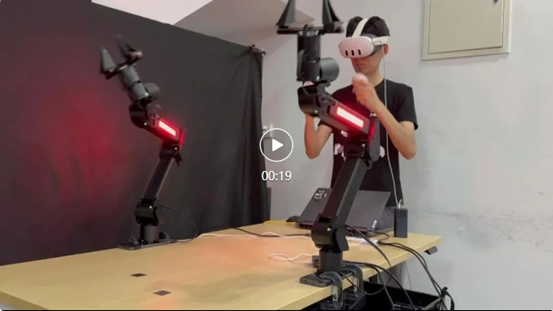
\includegraphics[width=0.6\linewidth]{Demo.png}
    \caption{Demo}
\end{figure}
In addition, the following figure roughly describes the final environment of our project, and briefly introduces the modules.
\begin{figure}[H]
    \centering
    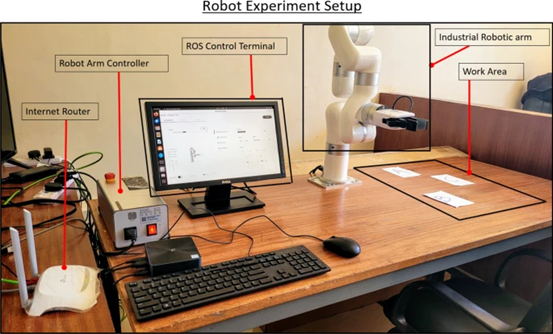
\includegraphics[width=0.6\linewidth]{Robot Experiment Setup.png}
    \caption{Experiment Setup}
\end{figure}
\section{High-level Requirements}
\begin{itemize}
    \item Successfully generate and import at least 10 digital twin objects into Virtual Reality. 
    \item The system should accurately map hand trajectory to robotic arm movements in real-time. 
    \item The robotic arm should replicate the grasping motion within 2 minutes of user interaction. 
\end{itemize}
\chapter{Design}

\section{Block Diagram}
\begin{figure}[H]
    \centering
    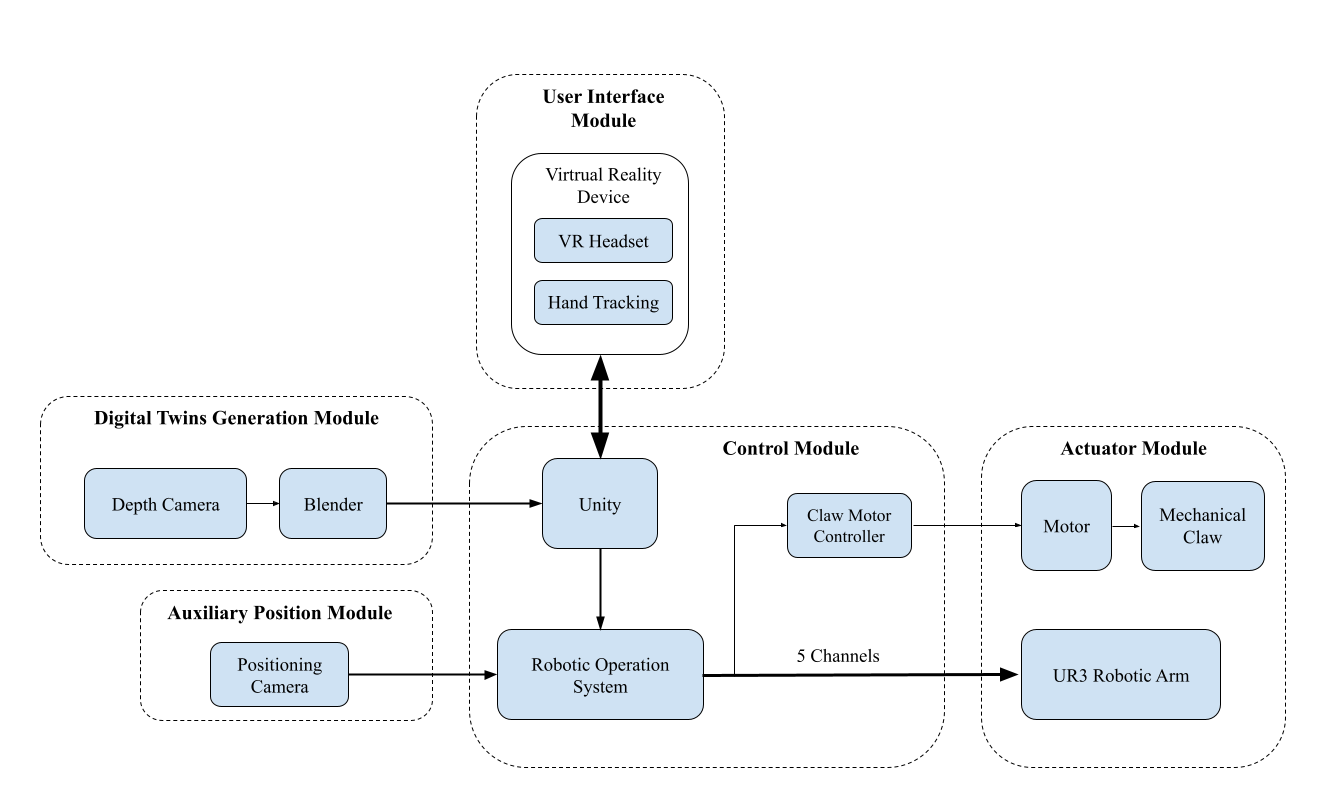
\includegraphics[width=1.0\linewidth]{Block Diagram.png}
    \caption{Block Diagram}
\end{figure}
\section{Physical Design}
Since the original robotic arm realizes picking up and placing objects through 
the suction force of suction cups, this limits the accuracy and fineness of 
gripping objects. Therefore, we decided to create a suitable mechanical claw 
through 3D modeling and control the motor to drive the mechanical claw to clamp
, thus replacing the operation of the suction cup. We believe that this will 
dramatically increase the level of maneuverability and reduce the requirements 
for the material and shape of the object to be gripped. The following figure shows
our design model of claw.
\begin{figure}[H]
    \centering
    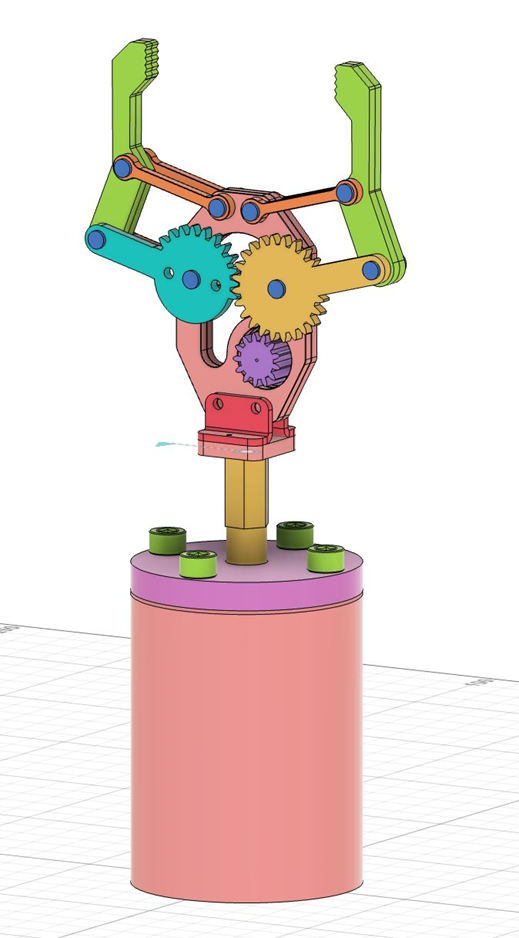
\includegraphics[width=0.4\linewidth]{Claw.png}
    \caption{Claw Model Design}
\end{figure}
\section{Subsystem Introduction}
\subsection{Digital Twins Subsystem}
\subsubsection*{Subsystem Description}
The Unity3D Digital Twin Subsystem provides a real-time 3D virtual replica of 
the physical system, using the Unity game engine to simulate and visualize the 
system's state. Its primary purpose is to mirror the physical equipment's 
behavior in a virtual environment for monitoring and operator interaction. 
The subsystem integrates Unity's physics engine and high-fidelity graphics 
rendering to model motions, forces, and object interactions that closely 
resemble the real world​. This digital twin receives live data from the physical 
system via a communication interface and updates the virtual model accordingly, 
thereby maintaining synchronization with the real equipment in near real-time. 
Within the overall system architecture, the Unity3D Digital Twin acts as the 
visualization and simulation layer. The Unity3D subsystem consumes these updates 
and applies them to the virtual model. In turn, the digital twin can also produce 
outputs or events​. This interaction enables scenarios like virtual commissioning 
and operator training, where the digital twin not only mirrors the physical 
system but can also influence it under controlled conditions. By leveraging 
Unity’s deployment, the digital twin visualization can run on operator VR 
headsets. 
\subsubsection*{Subsystem Requirements}
\textbf{Real-Time Visualization Performance:} The subsystem shall provide a smooth 
real-time visualization of the physical system. It must maintain a frame rate 
of at least 30 frames per second (FPS) during normal operation, with a target 
of 60 FPS for optimal smoothness.
\\
  
\textbf{Data Throughput and Update Rate:} The Unity3D subsystem shall handle incoming 
data streams from the physical system at a sufficient rate. It must support at 
least 10 Hz update frequency for all critical sensor inputs, matching the data 
acquisition rate of the system​. 
\\
  
\textbf{Scene Complexity and Rendering Capability:} The subsystem shall support the full 
complexity of the system's 3D model and environment. It must render all relevant 
components with high visual fidelity, including using imported CAD models for 
accuracy​. 
\\
  
\textbf{Integration and Compatibility:} The Unity3D subsystem must integrate seamlessly 
with the overall system's data and control architecture. It shall support 
standard industrial communication protocols or APIs provided by the system 
integrator. 
\subsubsection*{Subsystem Verification}
\textbf{Frame Rate Performance Test:} Set up a full-scale virtual scene in Unity that 
represents the complete physical system. Run the digital twin application on 
the target hardware under typical operating conditions. Use Unity's built-in 
frame timing stats to record the frame rate. Verification criteria: The 
measured frame rate should stay ≥30 FPS for 95\% of the samples. 
\\
  
\textbf{Accuracy Validation Test:} To verify the physical fidelity, we will compare 
the digital twin's reported state against the real system's state under 
controlled motions. We will record the corresponding position of the virtual 
model in Unity (the transform values or angles of the virtual joints). If a 
robot arm moves through 90°, the Unity twin's arm should be within range at 
all times. We will specifically check the worst-case alignment at extreme 
positions and dynamic moves. 
\subsection{VR Subsystem}
\subsubsection*{Subsystem Description}
The Meta Quest (or Oculus Quest VR headset) App block enables Meta Quest users to interact with the digital twin scene. In the runtime, it receives user hand trajectory from real world input. Then it processes the information for object recognition and finally sends the object index as well as the hand trajectory to the unity digital twin\cite{ARXroboticsX2025}. 
\textbf{Input:}  
\begin{enumerate}
    \item \textbf{Predefined 3D Models and Configurations:} A set of digital models representing 10 objects, a table, and a robotic arm with an end-point gripper. These models are loaded at initialization.
    \item \textbf{Scale \& Spatial Arrangement Data:} Tolerances data ensuring that scale precision remains within less than a 5\% error margin and that objects are distinctly separated from the table.
\end{enumerate}
\textbf{Output:} 
\begin{enumerate}
    \item \textbf{Rendered Digital Twin Scene:} A virtual representation in Unity that mirrors the physical arrangement with the required precision. 
    \item \textbf{Visual Context Data:} The positioning data of each element (objects, table, robotic arm) used by the object recognition module to compare with user hand trajectories. 
\end{enumerate}
\subsubsection*{Subsystem Requirements}
$\bullet$ The predefined scene serves as a VR counterpart to our Digital Twin in Unity. It incorporates physical models of the following elements: 10 objects, table and robotic arm. 

 

\textbf{Requirements:} The elements in the scene must have less than 5\% precision tolerance in scales. The 10 objects must be viewed as separable entities from the table. The robotic arm could be simplified as a rigid body, but the end-point gripper must manifest the same level of detail with other elements. 
\\
 

$\bullet$ Hands Tracking module captures user hands trajectories and sends them to the Digital Twin in Unity via proprietary API databus1 and object recognition module in real time. This is the key element to enable human robot interaction and is implemented by Unity First-Hand Dependencies \cite{unity-firsthand}. 

 

\textbf{Requirements:} Must capture hand trajectory every 0.2 seconds. Must convert the trajectory data to unity-readable format.
\\
 

$\bullet$ Object Recognition module predicts which object the user is targeting based on hand trajectories and records the object is grasped. It constantly receives data from Hands Tracking module and reads the real-time object locations in the scene as input, and after processing it sends the “predicted\_object” data packet to the Digital Twin Unity via proprietary API databus 2. The prediction task is a classification problem on the 10 objects with input of a string of hand trajectory in the past 10 seconds. The code is written into Meta Quest App Build. 

 

\textbf{Requirement:} The classification task should be performed in a limited time, e.g. 0.2 seconds. The prediction result must be accurate as the user hand approaches close (within 10 cm) to the target object.  

 
\subsubsection*{Subsystem Verification}
\textbf{Scene Module:} 
\begin{enumerate}
    \item Validate that imported models maintain scale precision by running automated comparisons against defined dimensional tolerances. 
    \item Test that spatial relationships (i.e., object separability) are preserved. 
\end{enumerate}
 
\textbf{Hands Tracking:} 
\begin{figure}[H]
    \centering
    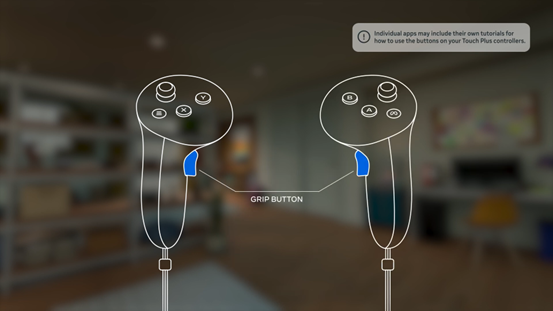
\includegraphics[width=0.6\linewidth]{Hands Tracking.png}
    \caption{Hands Tracking}
\end{figure}
\begin{enumerate}
    \item Simulate sensor inputs to ensure that trajectory data is sampled exactly every 0.2 seconds\cite{Gichane2024}. 
    \item Check correct conversion routines by comparing raw sensor data to Unity-compatible data formats. 
\end{enumerate}
 
\textbf{Object Recognition:} 
\begin{enumerate}
    \item Use synthetic trajectory data covering typical usage (including cases when the hand is within 10 cm of an object) to verify that classification returns the correct object index. 
    \item Measure processing time to confirm that prediction completes within the 0.2-second window. 
\end{enumerate}
 
\textbf{Integrated Testing:}
\begin{enumerate}
    \item Simulate the digital twin in Unity to receive and correctly interpret both hand trajectory and object recognition outputs via their respective data buses (Databus1 and Databus2)\cite{MirCore2025}. 
    \item Introduce simulated delays or corrupted data in sensor inputs to verify that error handling protocols are initiated and logged. 
\end{enumerate}
\subsection{Mechanical Arm Subsystem}
\subsubsection*{Subsystem Description}
The mechanical claw subsystem serves as the end-effector of the UR3 robotic arm, designed to enhance its ability to grasp small and irregularly shaped objects. Unlike the original suction-based unit, the claw uses a servo motor for independent actuation and provides improved adaptability to non-flat surfaces. The claw body is fabricated from laser-cut acrylic plates and assembled with M3 screws and nuts, allowing for quick prototyping and ease of maintenance. The subsystem mounts directly onto the UR3 flange and receives PWM control signals from the upper-level controller, enabling precise open-close motions. End-stop feedback sensors can be optionally integrated to provide closed-loop control. 
\subsubsection*{Subsystem Requirements}
This subsystem is fully student-designed and must comply with dimensional, functional, and performance constraints: 
\begin{figure}[H]
    \centering
    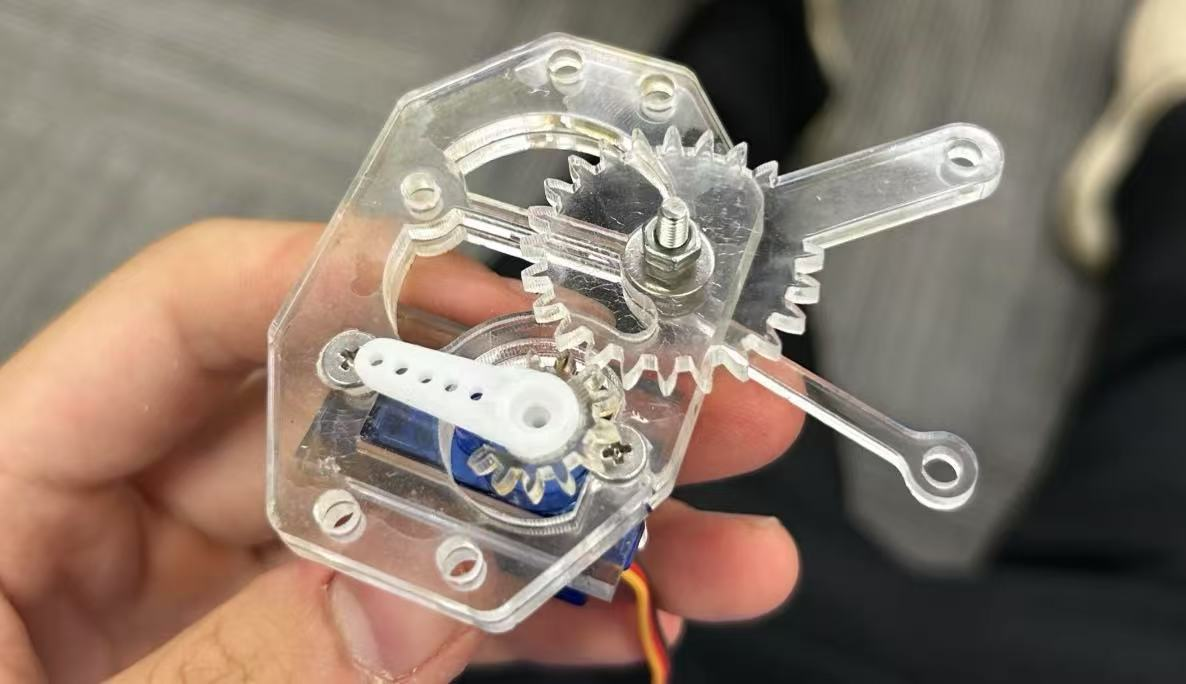
\includegraphics[width=0.6\linewidth]{Claw Test.png}
    \caption{Hands Tracking}
\end{figure}
\begin{itemize}
    \item \textbf{Size:} The claw must remain compact to fit within the working envelope of the UR3. The maximum allowable dimensions are 12 cm (length) × 10 cm (width). 
    \item \textbf{Gripping Range:} The claw should be capable of grasping objects with widths ranging from 0.8 cm to 6 cm, covering a broad range of daily-use items such as pens, keys, and bottle caps. 
    \item \textbf{Gripping Force:} A minimum holding force of 1.5 N is required to securely lift lightweight objects (~150g), assuming a friction coefficient of 0.4 between the gripper and object surfaces. 
    \item \textbf{Positioning Accuracy:} The maximum allowable misalignment during gripping is ±0.5 cm, necessitating adequate structural rigidity and low mechanical backlash. 
    \item \textbf{Material:} Lightweight and rigid materials must be used to minimize added load on the robotic arm. The current prototype uses 4 mm-thick acrylic plates. 
\end{itemize}
\subsubsection*{Subsystem Verification}
To verify that the claw meets performance and usability standards, the following test procedures will be conducted: 
\begin{itemize}
    \item \textbf{Grasping Tests:} The claw will attempt to grasp 10 different objects varying in size (0.8\–5 cm), shape (cylindrical, cubic, irregular), surface texture (smooth/rough), and mass (30–150 g). 
    \item \textbf{Holding Stability:} Each object will be held stationary for 5 seconds post-grasp. Success is defined as no slippage or drop.     
    \item \textbf{Repeatability Test:} Each grasping action will be repeated 10 times, with a target success rate of ≥90\% to ensure consistent performance. 
    \item \textbf{Durability Check:} After 100 grasp-release cycles, structural integrity and gripping force will be reevaluated. 
\end{itemize}
\section{Tolerance Analysis}
\subsection{Power Supply}
\subsubsection{UR3 Robotic Arm}
The UR3 typically operates on a 24V DC power supply. The current drawn by the robotic arm varies depending on the motion and the load. Under typical operating conditions, the current draw can be around 3-6 A, which means the maximum power consumption can peak at around 150-200 W. We need to use a satisfied DC source or designed AC-DC converter. 
\subsubsection{STM32 Chip}
We will use STM32F4 series chips to control the claw motor, which needs a 5V DC voltage to power. Therefore, there should be a transformer before using the 6th signal of UR3 as input of STM32.  
\subsection{UR3 Precision}
There are limitations to robotic UR3, ensuring that it can accurately move 
following the computed route. Motivation speed is one of the most important 
factors. As mentioned in the instruction document, the general speed tolerance 
is -150mm/s. This means that if the user configures a 250mm/s speed limit, then 
the maximum operational speed will be 250-150=100mm/s. Safety tolerances 
prevent safety violations while allowing for fluctuations in program behavior. 
For example, when handling a heavy payload, there may be situations where the 
Robot Arm needs to briefly operate above the normal maximum operational speed to 
follow a programmed trajectory \cite{ur3-manual}. An example of such a situation is shown in 
figure. 
\begin{figure}[H]
    \centering
    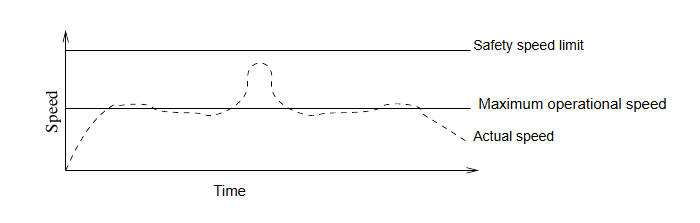
\includegraphics[width=0.8\linewidth]{UR3 Tolerance.png}
    \caption{Safety Tolerance Example}
\end{figure}
\subsection{Mechanical Claw}
A preliminary tolerance analysis focuses on the relationship between servo 
rotation and claw tip displacement. Based on linkage geometry, a ±$2^{\circ}$ servo 
error translates to approximately ±1.2 mm positional error at the gripper tips. 
The system’s performance is not highly sensitive to this variation, but finer 
control can be achieved by increasing servo resolution or using stiffer 
linkages. 
\subsection{Torch of Grasping}
The precision of grasping, especially whether the claw could successfully hold 
on to the items, mostly relies on the force of the claw applied. In other words, 
it depends on the torch range that the motor could supply. To verify the 
feasibility of our design, we want to use FEA ( Finite Element Analysis) 
method. Based on the shape, size, and material properties of the gripper’s 
fingers and the geometry of the object being grasped, combine this information 
with the 3D model of the claw to construct the model in FEA software, like 
ANSYS, COMSOL, or Abaqus. Use Static or Dynamic analysis to simulate contact 
pressure and displacement. With this information, we could get an appropriate 
torch. For example, the object material is plastic and can obtain 60 MPa 
maximum stress before damage. The friction coefficient ($\mu$) is 0.3. After 
simulation, we find we need to apply 15N force on the object, the contact area 
is $3mm^2$, according to the formula: 
\begin{equation*}
    Pressure(P)=\frac{Force(F)}{Area(S)}=\frac{15}{3} \cdot 10^{-6}=5MPa<60MPa 
\end{equation*}

We could ensure claw will not break the object if grasped successfully. Therefore, we could compute the corresponding Torch(T) with formula: 
\begin{equation*}
    Torch(T)=Length(L) \times Force(F)
\end{equation*} 
\chapter{Cost \& Schedule}
\section{Cost Analysis}
\begin{table}[H]
    \centering
    \renewcommand{\arraystretch}{1.5}
    \label{Cost-table}
    \begin{tabular}{|l|l|l|}
        \hline
        \textbf{Description}         & \textbf{Quantity}  & \textbf{Price} \\ 
        \hline
        STM32F407ZGT6 development board     & 1          & \textyen 174.08      \\
        \hline
        Emm42\_V5.0 motor control board     & 1          & \textyen 54.99      \\
        \hline
        42mm Stepper motor         & 1          & \textyen 22.99      \\
        \hline
        220V to 24V power supply & 1 & \textyen 19.80    \\ 
        \hline
        \textbf{\textit{Total}}         & \textbf{\textit{4}}  & \textbf{\textit{\textyen 271.86}} \\
        \hline
    \end{tabular}
\end{table}
\section{Schedule}

\begin{longtable}{|p{0.1\textwidth}|p{0.45\textwidth}|p{0.45\textwidth}|}
    \caption{Schedule of Y\&H} \label{longtable1} \\  % 表格标题
    \hline
    \textbf{Week} & \textbf{Yuchen Yang} & \textbf{Jingxing Hu} \\  % 表格头部
    \hline
    \endfirsthead  % 第一页表头

    % \hline
    % \multicolumn{3}{|c|}{\textit{Continued from previous page}} \\  % 翻页时表头标记
    \hline
    \textbf{Week} & \textbf{Yuchen Yang} & \textbf{Jingxing Hu} \\  % 表头重复
    \hline
    \endhead  % 后续页表头

    \hline
    \endfoot  % 页脚(例如,每页底部)

    \hline
    \multicolumn{3}{|c|}{\textit{End of the Table}} \\  % 最后一页的底部标记
    \hline
    \endlastfoot  % 最后一页的表格内容
    \hline
    1 
    
    &Research digital twin implementations; Unity3D physics and rendering 
    
    &Research servo motors, material strength, and existing claw designs 
    \\
    \hline
    2 
    
    &Design digital twin architecture and plan Unity3D scene structure 
    
    &Sketch CAD prototype and finalize hardware design plan 
    \\
    \hline
    3 
    
    &Set up Unity3D project; add initial 3D models; simulate physics 
    
    &Start CAD modeling; prepare for 3D printing claw prototype 
    \\
    \hline
    4 
    
    &Test 3D models in Unity; evaluate frame rate under load 
    
    &3D print initial claw prototype; test motor response via PWM 
    \\
    \hline
    5 
    
    &Implement mock data sync in Unity; evaluate real-time updates 
    
    &Assemble mechanical claw and test gripping control 
    \\
    \hline
    6 
    
    &Refine data handling pipeline; begin simulating real sensor inputs 
    
    &Improve grip stability; calibrate servo control logic 
    \\
    \hline
    7 
    
    &Add Unity interactivity: real-time movement and collision 
    
    &Strengthen claw design; begin durability tests 
    \\
    \hline
    8 
    
    &Run full-scene FPS test (>30 FPS goal); optimize lighting \& physics 
    
    &Test for accuracy and repeatability of claw motion 
    \\
    \hline
    9 
    
    &Sync Unity with physical data feed (prototype) 
    
    &Refine motor PID control; test with various object weights 
    \\
    \hline
    10 
    
    &Finalize Unity visuals; polish data update logic 
    
    &Final mechanical refinements; noise and fault tolerance 
    \\
    \hline
    11 
    
    &Document architecture; prepare demo scenes 
    
    &Document claw testing (grip force, speed, durability) 
    \\
    \hline
    12 
    
    &Present digital twin; live demo with physical hardware 
    
    &Present mechanical claw demo; handle various objects 
    \\
    \hline
\end{longtable}





\begin{longtable}{|p{0.1\textwidth}|p{0.45\textwidth}|p{0.45\textwidth}|}
    \caption{Schedule of Z\&Y}\label{longtable2} \\  % 表格标题
    \hline
    \textbf{Week} & \textbf{Jiayu Zhou} & \textbf{Ziming Yan} \\  % 表格头部
    \hline
    \endfirsthead  % 第一页表头

    % \hline
    % \multicolumn{3}{|c|}{\textit{Continued from previous page}} \\  % 翻页时表头标记
    \hline
    \textbf{Week} & \textbf{Jiayu Zhou} & \textbf{Ziming Yan} \\  % 表头重复
    \hline
    \endhead  % 后续页表头

    \hline
    \endfoot  % 页脚(例如,每页底部)

    \hline
    \multicolumn{3}{|c|}{\textit{End of the Table}} \\  % 最后一页的底部标记
    \hline
    \endlastfoot  % 最后一页的表格内容
    \hline

1 

&Research Meta Quest hand tracking \& interaction methods 

&Research communication protocols \& Unity-hardware integration 
\\
\hline
2 

&Outline VR app structure and flow 

&Plan subsystem integration, define performance benchmarks 
\\
\hline
3 

&Begin Unity-based VR scene setup; connect Meta Quest 

&Reproduce basic Unity-to-hardware data exchange 
\\
\hline
4 


&Implement basic hand tracking in Unity with Meta Quest 

&Set up data streaming and simulate sensor input flow 
\\
\hline
5 

&Start object recognition based on hand trajectory 

&Integrate hand tracking data with Unity interface 
\\
\hline
6 

&Optimize hand-object interaction tracking 

&Assist with feedback loop between claw and digital twin 
\\
\hline
7 


&Add object selection via gestures; refine visuals 

&Start working on system-wide debug tools and logs 
\\
\hline
8 

&Test multi-object interaction; debug recognition failures 

&Support VR-to-claw communication path and timing issues 
\\
\hline
9 

&Conduct usability tests with interaction gestures 

&Run full integration test across Unity, VR, claw 
\\
\hline
10 


&Finalize app flow; ensure smooth transitions 

&Debug bottlenecks in inter-subsystem latency 
\\
\hline
11 

&Record usage guide \& walkthrough video 

&Compile integration documentation and stability metrics 
\\
\hline
12 

&Present VR interaction demo; gesture to object pipeline 

&Support final system presentation and live testing 
\\
\hline
\end{longtable}
% \end{tabularx}
% \end{table}
\chapter{Ethics \& Safety}
\section{Ethics} 
In our project, the subsystem of the mechanical jaws is referenced from Raunak Jain's design in his October 2024 release of the Grabcad project \cite{Jain2024}. Various aspects of the structure and dimensions of this design were borrowed by us and suitably modified to suit the actual needs. However, in order to comply with the IEEE Code of Ethics 5 “Honest and Accurate Technical References”, we have ensured that all references in the project are labeled with the technical source and the original author in order to avoid any form of plagiarism or misrepresentation. Failure to cite these sources correctly could violate the IEEE Code of Ethics, compromise academic integrity, and undermine the credibility of the technical research. 
 
Realizing this, we have made further innovations to the design in the following areas: 
\begin{enumerate}
    \item \textbf{Design adaptability improvements:} In order to adapt the mechanical jaws to laser cut acrylic sheet processing, we fine-tuned the dimensions and tolerances of the original design. This adjustment ensures that the design is able to achieve a higher level of accuracy during the laser cutting process and guarantees processing efficiency. This adaptability improvement makes our design more in line with what is needed in actual production. 
    \item \textbf{Optimization of the rudder assembly:} Although the core structure of the servo assembly remains the same, we have optimized its components and assembly method. By reasonably adjusting the connection between the servo and the robotic arm, we have effectively improved the stability and operating precision of the mechanical gripper to ensure that it can better perform its tasks in practical applications. 
    \item \textbf{Innovation on manufacturing process:} Based on the original design, we have optimized the structure of the gripper jaws by combining the laser cutting process, especially in the selection of materials and processing methods. This not only effectively reduces the manufacturing cost, but also improves the overall strength and reliability of the part, adapting to different production requirements. 
    \item \textbf{Technical realization and applicability:} Our design not only focuses on the feasibility of technical realization, but also takes special consideration of the need for mechanical gripping jaws in smart home scenarios. Through these innovations, we have ensured that the gripper jaws are able to perform gripping tasks stably and efficiently when providing assistance to the physically challenged, while at the same time possessing a high degree of adaptability to suit the needs of use in different environments. 
\end{enumerate}
 
Through these innovations, we have not only compensated for the limitations of our reference work, but have also improved the overall performance and applicability of our mechanical grippers. These improvements reflect our efforts to build on the designs of others while adhering to the IEEE Code of Ethics \cite{IEEE} to ensure integrity and innovation in design. 
\section{Safety} 

Working in an electronics lab presents some challenges of its own. After rigorous safety training, we use laser cutters to cut and process acrylic sheets to avoid the risk of burns, electric shocks and inhalation of toxic fumes. Safety training was also carried out when operating the UR3 robotic arm to ensure that the arm operated within safe limits, avoiding malfunctions and ensuring the safety of those around it. 
 
For fixing and connecting the parts, we used screws and nuts and 502 glue bonding. As 502 glue is a kind of quick-drying glue, it is very easy to stick to the hand, in order to avoid this kind of safety hazards and facilitate the assembly, when bonding multiple acrylic panels together, we firstly use the screws to fix the position of the workpiece, and then use the rat-tailed needle to point on a small amount of 502 glue. 
 
When laser cutting smaller parts, it is easy to generate heat buildup, so we first verify whether the speed and power settings of the laser cutting machine are reasonable through simple graphic cutting, to avoid incomplete cutting leading to large errors, or too much power to cause fire. Before cutting, we will carefully check the design documents to avoid excessive concentration of heat due to repetitive alignment. During the cutting process, we observe the laser cutter throughout and are always ready to respond to possible failures. After cutting, we do not take out the acrylic sheet immediately, but turn off the laser cutting machine first, wait for the exhaust gas to be exhausted and the sheet to cool down, and then finally take out the finished cut parts. 
%%%%%%%%%%%%%%%%%%%%%%%%%%%%%%%%%%%%%%%%%%%%%%%%%%%%%%%%%%%%%%%%%
\clearpage
%%%%%%%%%%%%%%%%%%%%%%%%%%%%%%%%%%%%%%%%%%%%%%%%%%%%%%%%%%%%%%%%%
\backmatter
%%% References %%%%%%%%%%%%%%%%%%%%%%%%%%%%%%%%%%%%%%%%%%%%%%%%%%
\clearpage
\renewcommand*{\UrlFont}{\rmfamily}
\printbibliography[title={References},heading=bibintoc]
\clearpage
%%%%%%%%%%%%%%%%%%%%%%%%%%%%%%%%%%%%%%%%%%%%%%%%%%%%%%%%%%%%%%%%%
\end{document}